\documentclass[twoside, a5paper]{article}
\RequirePackage[top=0.5in,left=0.5in,right=0.5in,bottom=0.5in,includefoot]{geometry}
\usepackage[latin,english]{babel}


\usepackage[center]{titlesec}

\usepackage{afterpage}
\usepackage{multicol}
% \usepackage{showframe} only for check block positions
%\usepackage[margin=3cm]{geometry}
\usepackage{paracol}
\setlength{\columnsep}{1em}
\footnotelayout{m}

\usepackage[autocompile]{gregoriotex}
\usepackage{libertine}
\usepackage[center]{titlesec}
\usepackage{csquotes}

%no section numbers
\renewcommand\thesection{}

\usepackage{textpos} % use "showboxes" for check results
\setlength{\TPHorizModule}{.1\textwidth} % = 10% width
\setlength{\TPVertModule}{.01\textheight}% = 01% height

% Facing Double Block Macro
% Usage: 
% \FDB{position}{section}{even text}{odd text}
% position = a number between 0 to 100 (or some less)

\newcommand\FDBS[4]{
\begin{textblock}{10}(0,#1)
%\textblockcolour{cyan!10} % ugly, only for testing
\section{#2\label{#2}} #3 \medskip 
\end{textblock}
\afterpage{
\begin{textblock}{10}(0,#1)
% \textblockcolour{green!10} % ugly, only for testing
\section*{#2}
 #4\smallskip
\end{textblock}}}

\newcommand\FDB[3]{
\begin{textblock}{10}(0,#1)
%\textblockcolour{cyan!10} % ugly, only for testing
 #2 \smallskip 
\end{textblock}
\afterpage{
\begin{textblock}{10}(0,#1)
% \textblockcolour{green!10} % ugly, only for testing
 #3\smallskip
\end{textblock}}}

\newcommand*{\red}[1]{\textcolor{red}{#1}}
\newcommand*{\redit}[1]{\textit{\textcolor{red}{#1}}}

\usepackage{changepage}
\newcommand{\prayer}[3][3em]{%
  \begin{adjustwidth}{#1}{0pt}%
    \makebox[0pt][r]{\makebox[#1][l]{\bfseries \redit{#2}}}%
    \ignorespaces #3
  \end{adjustwidth}
}

\makeatletter
\newenvironment{litany}
  {\list{\topsep=0pt}{%
   \setlength{\topsep}{0pt}%
   \setlength{\leftmargin}{2em}%
   \setlength{\listparindent}{-2em}%
   \setlength{\itemindent}{-2em}%
   \setlength{\parsep}{\parskip}}%
   \item[]}%
  {\endlist}
\makeatother

\newenvironment{nstab}
  {\setlength{\topsep}{-\parskip}%
   \setlength{\partopsep}{0pt}%
   \tabbing}
  {\endtabbing}

\usepackage[savepos]{zref}

\makeatletter  
\newcounter{score}
\newcounter{tabstop}[score]
\newcommand{\grealign}{%
	\@bsphack%
	\ifgre@boxing\else%
		\kern\gre@dimen@begindifference%
		\stepcounter{tabstop}%
		\expandafter\zsavepos{stop-\thescore-\thetabstop}%
		\kern-\gre@dimen@begindifference%
	\fi%
	\@esphack%
}

\newcommand{\setstops}{%
  \gdef\nstabbing@stops{%
    \hspace*{-\oddsidemargin}\hspace{-1in}%
    \hspace*{\zposx{stop-\thescore-1} sp}\=%
  }%
  \count@=\@ne
  \loop\ifnum\count@<\value{tabstop}%
    \begingroup\edef\x{\endgroup
      \noexpand\g@addto@macro\noexpand\nstabbing@stops{%
        \noexpand\hspace{-\noexpand\zposx{stop-\thescore-\the\count@} sp}%
        \noexpand\hspace{\noexpand\zposx{stop-\thescore-\the\numexpr\count@+1} sp}\noexpand\=%
      }%
    }\x
    \advance\count@\@ne
  \repeat
  \nstabbing@stops\kill
}
\makeatother

\newenvironment{nstabbing}
  {\setlength{\topsep}{-\parskip}%
   \setlength{\partopsep}{0pt}%
   \tabbing%
   \setstops}
  {\endtabbing\stepcounter{score}}

\usepackage{environ}
\makeatletter
\NewEnviron{firstnote}{
  \ifnum\gre@lastoflinecount=2
    \BODY
  \else
    \null
  \fi}
\makeatother


\begin{document}

\thispagestyle{empty}
\hspace{0pt}
\vfill

\begin{center}
\uppercase{\textbf{\huge ``Kleczki Jasnagorskie''}} \par
\vspace{1em}
\uppercase{\textbf{\large Litany \\ of \\ Our Blessed \\ Virgin Mary}} \par
\end{center}

\vfill

\begin{center}
Australia 2017 
\end{center}

\hspace{0pt}

\newpage

\noindent\textbf{Permission to be printed:}\\
\vfill

\noindent\textbf{Dedication:}\\
We, Brothers Joseph Maria and Casimir OSPPE, wish to dedicate this work in thanksgiving for the 25\textsuperscript{th} anniversary of the priestly ordination of our provincial, the Very Rev. Fr Jarosław Zań OSPPE. We wish to give thanks for his 25 years of priestly service, his example as monk of the order and his labours as the provincial of the Australian Province of the Order. 

\vfill

\noindent\textbf{Acknowledgements:}\\
This book was arranged by Br. Casimir Zielinski OSPPE and the music was type set by Fr. Joseph Maria Buckley OSPPE. We wish to thank Fr. Bazyli Degórski OSPPE in his assistance in translating \textit{O Maria Cna Dziwica}, likewise we to thank Fr. Nikodem Kilnar OSPPE for this support and encouragement. 
\medskip

Finally, we wish to thank Miss Catherine Letchford for providing the cover art and to acknowledge the use of drawings of Fr. Augustine Pelnaowski OSPPE.

\newpage

\tableofcontents

\newpage 

\section{The Pauline Chant Project}

\setlength{\parskip}{1em}

No one can picture or imagine monks or monasteries without sacred chant being sung. Gregorian chant is intimately bound up with and associated not only with the Monastic life, but also with the Liturgy itself. Vatican II has this to say about Gregorian Chant.

\begin{displayquote}
\textit{112. The musical tradition of the universal Church is a treasure of inestimable value, greater even than that of any other art. The main reason for this pre-eminence is that, as sacred song united to the words, it forms a necessary or integral part of the solemn liturgy\ldots}

\textit{Therefore sacred music is to be considered the more holy in proportion as it is more closely connected with the liturgical action, whether it adds delight to prayer, fosters unity of minds, or confers greater solemnity upon the sacred rites.}

\textit{116. The Church acknowledges Gregorian chant as specially suited to the Roman liturgy: therefore, other things being equal, it should be given pride of place in liturgical services.}
\end{displayquote}

\hfill\textit{Sacrostancum Concilium, Vatican II’s document on the Liturgy}

It may come as a surprise to many; Gregorian chant once had many different expressions and forms. Each order had its own particular flavour and melodies of the same chants. The Pauline order was no different. In fact, Fr. Nikodem Kilnar OSPPE, the Chaplain of the Polish Bishop’s conference to Polish Church musicians, makes the bold claim that the Chant of the Pauline order was once better than that of the Benedictines.

Unfortunately, due to the near eradication of the Order in the 19th Century and the difficulties of the 20th century, the Order has lost much of its repertoire and practice. There is an effort in the Order at the moment, spearheaded by Fr Nikodem Kilnar to restore and promote the proud and unique chant traditions of the Order.
The Australian Province with the generous assistance of the Australia Sacred Musicians Association (ASMA) is in the process of promoting, recording and making this Pauline chant project accessible to the English-speaking world.

This presentation of the Kneeling prayers of Jasna Góra, hopes to make this precious Pauline devotion available to the English speaking Provinces and Houses of the Order as well as to English speaking pilgrims and parishioners.

\subsection*{What are the Kneeling prayers of Jasna Góra?}

The 1800’s saw the great order of St Paul the Frist Hermit titter on the brink of annihilation. The Order saw the many flames of the sons of St Paul and Blessed Eusebius reduced to just two, the monasteries of Skałka and Jasna Góra. These were were the only houses of the order left in the world and even they were in danger of being snuffed out.

Worse still, Jasna Góra, ultimately found itself in the Russian partition of Poland and was forced to wear a heavy Tsarist yoke. The Cloister was abolished, with pilgrims living and rummaging through monastic cells. The precious Lay Brothers were ejected and abolished. New Vocations had to jump through rigorous hoops created by the state. The common life was forcibly stopped. Above all, the public choral office was forbidden, a heavy and venomous blow to the heart of the monastic life! 

The Monks of Jasna Góra did not fall or give up under such a heavy yoke, attacking the very fundamentals and \textit{raison d'etre} of monastic life. No the monks outsmarted their overlords and oppressors. Gathering in the Black Madonna Chapel, before the very gaze of the Queen of Poland, the monks met together, not to chant the contraband divine office, but rather to chant devotions, liturgical devotions. 

\textit{Klęczki} or the Kneeling prayers of Jasna Góra, are not liturgy, but a selection of beautiful prayers and chants of the ancient order, under the mantle of a devotion. \textit{Klęczki} are composed of  8 parts. Firstly the monks chanted the litany of the Blessed Virgin Mary, invoking her as the Mother of the Order and Queen of Hermits, according to the melody proper to Jasna Góra. Secondly, the monks, fled to under her protection in the \textit{Sub Tuum}. Thirdly the monks implored her to show herself to be their mother, with the hands confidently outstretched in a haunting melodic version of the fourth stanza of the \textit{Ave Maris Stella}. After which follow a series of vesicles and responses asking God to send help from on high. Next are several collects. In the medieval ages, the collects of Mass were prayed in odd sets, either, one, five or seven, depending on the need. Here the monks prayed a full set of seven collects, for peace, for rain, for protection against their enemies and for a happy death. They did this using the melody proper to the order. 

Crowning these prayers, the monks chanted the first verse, in old Polish, of a hymn to the Queen of Poland. This booklet, following the mind and example of the late Father Augustine Lazur has translated it into Latin, to make it accessible to all. Psalm 130, as a vestige of the glorious choral office of the order is sung, expressing the cry of the monks in the depths of their troubles.  Lastly, the Monks hail Our Lady as their Queen in the Solemn \textit{Salve Regina}, again, using their ancient melody. 

The Kneeling prayers come from a very dark and stormy time in the history of the Order, but they also preserve the radiant glory of the patrimony of the Order. As one of my confreres from novitiate commented, ``\textit{Certainly these prayers helped perverse the order from extinction.}''

It is our hope that these prayers once again resound in our houses and monasteries. This book aims to assist their use and their spread not only amongst our monks, but also to our English-speaking parishioners and pilgrims.

\vfill
\begin{flushright}
Br Casimir Zielinski OSPPE \\
The Feast of Our Lady Queen of Poland \\
The 3rd of May 2017 \\
Prima Porta, Rome
\end{flushright}

\newpage 

\section{Rubrics}

Since the kneeling prayers are not an official liturgy of the church, but a form of devotion of the order, it is difficult to imagine set and definite rubrics. Nevertheless, there are two suggested forms. The first form, which may be used as an internal devotion of the order, may form a part of the weekly horarium of a house or monastery, and is prayed in the choir or chapel of the order. The second form, on the other hand, is suggested for public use, with the faithful and with more solemnity, in the church of our parish, house or monastery. 

\subsection*{\red{The First Form}}

\red{The monks gather in the chapel or arrive there in procession from the refectory. Taking their places in choir, they kneel down and following a sign from the superior, the cantor begins the litany.  The seven collects may be divided among various monks, but the superior chants the final collect, following the Salve.}

\red{As this is not a liturgy, no stole needs to be worn by the superior.}

\subsection*{\red{The Second Form}}

\red{Slightly before the commencement of the prayers, the community gathers in the sacristy. It is highly encouraged that those who can wear the mantle and thus the full habit of the order, do so. The community processes out into the church and take their place according to profession and precedence, either in their stalls or before the Icon of Our Lady of Jasna Góra solemnly exposed for veneration.  Once all are ready, the Cantor or cantors begin the Litany. The seven collects may be divided among various monks, but the superior chants the final collect, following the Salve.}

\red{As this is not a liturgy, no stole needs to be worn by the superior, but for the sake of the faithful, the superior may wear one. It would be appropriate to offer a word of introduction, perhaps with a sign of the cross and a greeting,  before the cantors begin the litany. Likewise, after the final collect, it would be appropriate to bless the people and dismiss them.}

\setlength{\parskip}{0pt}

\newpage

\section{Litany of Our Lady}

\gresetlastline{justified}
\gresetinitiallines{0}
\gresethyphen{force}
\gregorioscore{../music/kyrie-i}%
\begin{nstabbing}%
\>Fi-\>li, Redemptor mundi \>De-\>us,\\
\>Spi-\>ritus Sancte \>De-\>us,\\
\>San-\>cta Trinitas, unus \>De-\>us,\\
\end{nstabbing}
\gregorioscore{../music/kyrie-ii}
\medbreak

\prayer{\Vbar.}{Lord, have mercy on us.}
\prayer{\Rbar.}{Christ, have mercy on us.}
\prayer{\Vbar.}{Christ, hear us.}
\prayer{\Rbar.}{Christ, graciously hear us}
\prayer{\Vbar.}{God the Father of heaven, \hfill \red{\Rbar.} \textbf{Have mercy on us.}}
\hspace*{3em}God the Son, Redemmer of the world \\
\hspace*{3em}God the Holy Spirit \\
\hspace*{3em}Holy Trinity, one God,
\prayer{\Vbar.}{Holy Mary, \hfill \red{\Rbar.} \textbf{Pray for us}}

\medbreak

\underline{Sa}ncta Dei \underline{Ge}netrix,\hspace*{\fill}  Holy Mother of God,\par
\underline{Sa}ncta Virgo \underline{vi}rginum, \hspace*{\fill} Holy Virgin of virgins,\par
\underline{Ma}ter \underline{Chri}sti, \hspace*{\fill} Mother of Christ,\par
\underline{Ma}ter Ecc\underline{les}iae, \hspace*{\fill} Mother of the Church,\par
\underline{Ma}ter Ordinis \underline{no}stri \hspace*{\fill} Mother of Our Order,\par
\underline{Ma}ter Divinae \underline{gra}tiae, \hspace*{\fill} Mother of divine grace,\par
\underline{Ma}ter pu\underline{ris}sima, \hspace*{\fill} Mother most pure,\par
\underline{Ma}ter cas\underline{tis}sima, \hspace*{\fill} Mother most chaste,\par
\underline{Ma}ter invio\underline{la}ta, \hspace*{\fill} Mother inviolate,\par
\underline{Ma}ter inteme\underline{ra}ta, \hspace*{\fill} Mother undefiled,\par
\underline{Ma}ter a\underline{ma}bilis, \hspace*{\fill} Mother most amiable,\par
\underline{Ma}ter admi\underline{ra}bilis, \hspace*{\fill} Mother of good counsel,\par
\underline{Ma}ter boni Con\underline{si}lii, \hspace*{\fill} Mother of our Creator,\par
\underline{Ma}ter Crea\underline{to}ris, \hspace*{\fill} Mother of our Saviour,\par
\underline{Ma}ter Salva\underline{to}ris, \hspace*{\fill} Virgin most prudent,\par
\underline{Vir}go pruden\underline{tis}sima, \hspace*{\fill} Virgin most venerable,\par
\underline{Vir}go vene\underline{ran}da, \hspace*{\fill} Virgin most renowned,\par
\underline{Vir}go praedi\underline{can}da, \hspace*{\fill} Virgin most powerful,\par
\underline{Vir}go \underline{po}tens, \hspace*{\fill} Virgin most merciful,\par
\underline{Vir}go \underline{cle}mens, \hspace*{\fill} Virgin most faithful,\par
\underline{Vir}go fi\underline{de}lis, \hspace*{\fill} Mirror of justice,\par
\underline{Spe}culum iu\underline{sti}tiae, \hspace*{\fill} Seat of wisdom,\par
\underline{Cau}sa nostrae lae\underline{ti}tiae, \hspace*{\fill} Cause of our joy,\par
\underline{Vas} spiritu\underline{a}le, \hspace*{\fill} Spiritual vessel,\par
\underline{Vas} hono\underline{ra}bile, \hspace*{\fill} Vessel of honour,\par
\underline{Vas} insigne devoti\underline{o}nis, \hspace*{\fill} Singular vessel of devotion,\par
\underline{Ro}sa \underline{my}stica, \hspace*{\fill} Mystical rose,\par
\underline{Tur}ris Da\underline{vi}dica, \hspace*{\fill} Tower of David,\par
\underline{Tur}ris e\underline{bur}nea, \hspace*{\fill} Tower of ivory,\par
\underline{Do}mus \underline{au}rea, \hspace*{\fill} House of gold,\par
\underline{Foe}deris \underline{ar}ca, \hspace*{\fill} Ark of the covenant,\par
\underline{Ia}nua \underline{cae}li, \hspace*{\fill} Gate of heaven,\par
\underline{Ste}lla matu\underline{ti}na, \hspace*{\fill} Morning star,\par
\underline{Sa}lus infir\underline{mo}rum, \hspace*{\fill} Health of the sick,\par
\underline{Re}fugium pecca\underline{to}rum, \hspace*{\fill} Refuge of sinners,\par
\underline{Con}solatrix afflic\underline{to}rum, \hspace*{\fill} Comforter of the afflicted,\par
\underline{Au}xilium Christia\underline{no}rum, \hspace*{\fill} Help of Christians,\par
\underline{Re}gina Ange\underline{lo}rum, \hspace*{\fill} Queen of Angels,\par
\underline{Re}gina Patriar\underline{cha}rum, \hspace*{\fill} Queen of Patriarchs,\par
\underline{Re}gina Prophe\underline{ta}rum, \hspace*{\fill} Queen of Prophets,\par
\underline{Re}gina Aposto\underline{lo}rum, \hspace*{\fill} Queen of Apostles,\par
\underline{Re}gina \underline{Mar}tyrum, \hspace*{\fill} Queen of Martyrs,\par
\underline{Re}gina Confes\underline{so}rum, \hspace*{\fill} Queen of Confessors,\par
\underline{Re}gina Eremi\underline{ta}rum, \hspace*{\fill} Queen of Hermits,\par
\underline{Re}gina \underline{Vir}ginum, \hspace*{\fill} Queen of Virgins,\par
\underline{Re}gina Sanctorum \underline{om}nium, \hspace*{\fill} Queen of all Saints,\par
\underline{Re}gina sine labe originali con\underline{cep}ta, \hspace*{\fill} Queen conceived without \par \hspace*{\fill} original sin,\par
\underline{Re}gina in caelum as\underline{sum}pta, \hspace*{\fill} Queen assumed into heaven,\par
\underline{Re}gina Sacratissimi Ro\underline{sa}rii, \hspace*{\fill} Queen of the most holy Rosary,\par
\underline{Re}gina famili\underline{a}rum, \hspace*{\fill} Queen of the family,\par
\underline{Re}gina \underline{pa}cis, \hspace*{\fill} Queen of Peace,\par
\underline{Re}gina \underline{Po}loniae \hspace*{\fill} Queen of Poland\par
\underline{Re}gina \underline{Mu}ndi \hspace*{\fill} Queen of the World\par
\underline{Mag}na Domina Hungar\underline{or}um \hspace*{\fill} Great Mistress of the Hungarians\par

\medbreak

\gregorioscore{../music/agnus-die}

\medbreak

\prayer{\Vbar.}{\textbf{Lamb of God who takes away the sins of the world.}}
\hfill\red{\Rbar.} Spare us, O Lord.
\prayer{\Vbar.}{\textbf{Lamb of God who takes away the sins of the world.}}
\hfill\red{\Rbar.} Graciously hear us, O Lord.
\prayer{\Vbar.}{\textbf{Lamb of God who takes away the sins of the world.}}
\hfill\red{\Rbar.} Have mercy on us.

\noindent
\includegraphics[width=\textwidth]{madonna}

\newpage

\FDBS{0}{Sub Tuum Praesidium}{\gregorioscore{../music/sub-tuum-praesidium}}{
\begin{center}
We fly to thy patronage, O holy Mother of God;

Despise not our petitions in our necessities,

But deliver us always from all dangers,

O glorious and blessed Virgin
\end{center}}

\FDBS{55}{Monstra Te}{\gregorioscore{../music/monstra-te}}{
\begin{center}
Show thyself to be a Mother:

Through thee may he receive prayer

Who, being born for us,

Undertook to be thine own
\end{center}}

\newpage\null\newpage

\section{Vesicles and Responses}

\gresetlastline{justified}
\gresetinitiallines{0}
\gresethyphen{force}

\FDB{0}{\gregorioscore{../music/versus-et-responsiones-i}}{
\vspace{2em}
\prayer{\Vbar.}{\textbf{In all our tribulations and difficulties.}}
\prayer{\Rbar.}{Help us, O Most Holy Virgin Mary.}
}

\gresetinitiallines{1}
\greillumination{ }
\FDB{30}{\gregorioscore{../music/versus-et-responsiones-ii}}{
\vspace{2em}
\prayer{\Vbar.}{\textbf{God arises; His enemies are scattered.}}
\prayer{\Rbar.}{And those who hate Him flee before Him.}
}

\greillumination{ }
\FDB{60}{\gregorioscore{../music/versus-et-responsiones-iii}}{
\vspace{2em}
\prayer{\Vbar.}{\textbf{Let peace be in thy strength:}}
\prayer{\Rbar.}{and abundance in thy towers.}
}

\newpage\null\newpage

\greillumination{ }
\FDB{0}{\gregorioscore{../music/versus-et-responsiones-iv}}{
\vspace{2em}
\prayer{\Vbar.}{\textbf{Help us, O God, of our salvation;}}
\prayer{\Rbar.}{and for the honour of thy name deliver us.}
}

\greillumination{ }
\FDBS{30}{Tempore aestivo}{\begin{center}(Pro serenitate vel pluvia)\end{center}
\gregorioscore{../music/versus-et-responsiones-v-i}
\begin{nstabbing}
\>II. pluviam \>con-\>gru-\>en-\>tem.
\end{nstabbing}
\gresetinitiallines{0}
\gregorioscore{../music/versus-et-responsiones-v-ii}}{
\prayer{\Vbar.}{\textbf{Lord give us I. Peace \\ \hspace*{5.5em} II. Coherent rain}}
\prayer{\Rbar.}{And the Earth will give us its fruit.}
\medbreak
\prayer{\Vbar.}{\textbf{O Lord, send us help from the sanctuary.}}
\prayer{\Rbar.}{And strengthen us out of Sion.}
}


\newpage\null\newpage

\section{The Seven Collects}

\begin{sloppypar}
\begin{paracol}{2}

\begin{otherlanguage}{latin}
Oremus: Defende quaesumus, Domine, Beata Maria semper Virgine intercedente istam ab omni adversitate familiam; et toto corde tibi prostratam, ab hostium propitius tuere clementer insidiis. 
\end{otherlanguage}

\switchcolumn

Do Thou, we beseech Thee, O Lord, by the intercession of Blessed Mary ever virgin, defend this family from all harm and mercifully deign to protect from the snares of the enemy, those who prostrate themselves before Thee.

\end{paracol}
\medbreak
\begin{paracol}{2}

\begin{otherlanguage}{latin}
II: Deus, qui conteris bella et impugnatores in te sperantium potentia tuae defensionis expugnas: auxiliare famulis tuis, implorantibus misericordiam tuam; ut inimicorum suorum feritate depressa, incessabili te gratiarum actio ne laudemus.\footnote{The collect for Masses in times of war, which may be found in  the 1962 Missal}
\end{otherlanguage}

\switchcolumn

O God, Who bringest wars to nought and shieldest by Thy power all who hope in thee, overthrowing those that assail them: help Thy servants who implore Thy mercy. So that thee fierce might of their enemies may be brought low, and we may never cease to praise and thank Thee.

\end{paracol}
\medbreak
\begin{paracol}{2}

\begin{otherlanguage}{latin}
III: Deus a quo sancta desideria, recta consilia et iusta sunt opera: da servis tuis illam quam, mundus dare non potest, pacem ut et corda nostra mandatis tuis dedita, et hostium sublata formidine, tempora sint, tua protectione tranquilla.\footnote{The collect for peace, which may be found in  the 1962 Missal}
\end{otherlanguage}

\switchcolumn

O God, from Whom are holy desires, right counsels, and just works: give to Thy servants, that which the world cannot give, both that our hearts may be disposed to obey Thy commandments, and also, the fear of enemies being removed, our times, by Thy protection, may be peaceful.

\end{paracol}
\medbreak
\begin{paracol}{2}

\begin{otherlanguage}{latin}
IV: Deus, misericordiae, Deus pietatis, Deus clementiae, qui misertus super afflictionem populi tui, dixisti angelo percutienti: Sufficit, nunc contine manum tuam ob amorem illius stellae gloriosae, cuius ubera praeciosa contra venenum delictorum nostrorum dulciter suxisti praesta auxilium gratiae tuae ut ab omni peste et improvida morte liberemur et a totius perditionis incursu misericorditer salvemur.
\end{otherlanguage}

\switchcolumn

God of Mercy, God of Piety, God of Clemency, who is merciful over the affliction of your people, you said to the destroying angel: enough now contain your arm. On account of the Love of that glorious star, who’s precious breast sweetly gave you suck against the venom of our sins;  grant the help of your grace, so that from all disease and sudden death we may be delivered and we may be mercifully saved from the attack of all perdition.

\end{paracol}
\medbreak

\redit{Here there is a choice of two prayers, either the first asking for peace or the seconding asking for rain.}
\medskip

\begin{paracol}{2}

\begin{otherlanguage}{latin}
V\textsuperscript{I}: Ad te nos, Domine, clamantes exaudi et aëris serenitatem tribue supplicantibus, ut qui iuste pro peccatis nostris affligimur, misericordia tua praeveniente clementiam sentiamus. 
\end{otherlanguage}

\switchcolumn

O Lord, hear us who cry to Thee, and grant fine weather to Thy suppliants, that we who are justly afflicted for our sins, may by the exercise of Thy bounty experience Thy clemency.\footnote{The collect for fair weather, which may be found in  the 1962 Missal}

\end{paracol}
\medbreak
\begin{paracol}{2}

\begin{otherlanguage}{latin}
V\textsuperscript{II}: Deus, in quo vivimus movemur et sumus, pluviam nobis tribue congruentem, ut praesentibus subsidiis sufficienter adiuti, sempiterna fiducialiter appetamus.\footnote{The collect for rain, which may be found in the 1962 Missal}
\end{otherlanguage}

\switchcolumn

O God, in Whom we live, move and have our being, grant us seasonable rain, that, our temporal needs being sufficiently supplied, we may with greater confidence seek after things eternal.

\end{paracol}
\medbreak
\begin{paracol}{2}

\begin{otherlanguage}{latin}
VI: Hostium nostrorum, quaesumus Domine elide superbiam; et eorum contumaciam dextere tuae virtute prosterne.\footnote{The collect against persecutors and evildoers, which may be found in the 1962 Missal.}
\end{otherlanguage}

\switchcolumn

O Lord, we beseech Thee, crush the pride of our enemies and humble their insolence by the might of Thy hand.

\end{paracol}

\end{sloppypar}
\medbreak

\begin{center}
\redit{All Seven prayers are concluded with one Conclusion.}
\end{center}
\medbreak

\gregorioscore{../music/per-christum}

\medbreak
\begin{paracol}{2}

\begin{otherlanguage}{latin}
Per Christum Dominium nostrum. Amen.
\end{otherlanguage}

\switchcolumn

Through Christ Our Lord. Amen.

\end{paracol}

\newpage

\FDBS{10}{O Maria Virgo Honesta}{\gregorioscore{../music/o-maria-virgo-honesta}}{\begin{center}Oh, Mary Honourable Virgin,

You have brought forth the king

The Heavenly heir

You brought him forth without sorrow,

Deliver us from sorrow and sadness

Hail Mary
\end{center}}

\newpage\null\newpage

\section{De Profundis}

\gresetinitiallines{0}
\gregorioscore{../music/de-profundis}
\medbreak

\begin{paracol}{2}
\begin{litany}
\begin{otherlanguage}{latin}
Fiant aures tuae intendéntes \red{*}\par
\hspace{1em}in vocem deprecationis meae.\par
\end{otherlanguage}
\end{litany}

\switchcolumn

\begin{litany}
Let your ears be attentive \red{*}\par
\hspace{1em}to the voice of my supplication\par
\end{litany}
\end{paracol}
\medbreak

\begin{paracol}{2}
\begin{litany}
\begin{otherlanguage}{latin}
Si iniquitátes observáveris, Domine, \red{*}\par
\hspace{1em}Domine, quis sustinébit.\par
\end{otherlanguage}
\end{litany}

\switchcolumn

\begin{litany}
If you, Lord, were to mark iniquities, \red{*}\par
\hspace{1em}who, O Lord, shall stand?\par
\end{litany}
\end{paracol}
\medbreak

\begin{paracol}{2}
\begin{litany}
\begin{otherlanguage}{latin}
Quia apud te propitiátio est, \red{*}\par
\hspace{1em}et timébimus te.\par
\end{otherlanguage}
\end{litany}

\switchcolumn

\begin{litany}
But with you is forgiveness, \red{*}\par
\hspace{1em}that you may be revered.\par
\end{litany}
\end{paracol}
\medbreak

\begin{paracol}{2}
\begin{litany}
\begin{otherlanguage}{latin}
Sustínui te, Domine: \red{\GreDagger}\par
\hspace{1em}sustínuit ánima mea in verbo eius, \red{*}\par
\hspace{1em}sperávit ánima mea in Domino.\par
\end{otherlanguage}
\end{litany}

\switchcolumn

\begin{litany}
I trust in the Lord: \red{\GreDagger}\par
\hspace{1em}my soul trusts in his word, \red{*}\par
\hspace{1em}My soul waits for the Lord.\par
\end{litany}
\end{paracol}
\medbreak

\begin{paracol}{2}
\begin{litany}
\begin{otherlanguage}{latin}
Magis quam custodes auroram, \red{*}\par
\hspace{1em}speret Israel in Domino.\par
\end{otherlanguage}
\end{litany}

\switchcolumn

\begin{litany}
More than watchmen wait for the dawn \red{*}\par
\hspace{1em}let Israel hope in the Lord.\par
\end{litany}
\end{paracol}
\medbreak

\begin{paracol}{2}
\begin{litany}
\begin{otherlanguage}{latin}
Quia apud Dominum misericordia, \red{*}\par
\hspace{1em}et copiosa apud eum redémptio.\par
\end{otherlanguage}
\end{litany}

\switchcolumn

\begin{litany}
For with the Lord there is mercy, \red{*}\par
\hspace{1em}and with him is plenteous redemption.\par
\end{litany}
\end{paracol}
\medbreak

\begin{paracol}{2}
\begin{litany}
\begin{otherlanguage}{latin}
Et ipse rédimet Israel \red{*}\par
\hspace{1em}ex omnibus iniquitátibus eius.\par
\end{otherlanguage}
\end{litany}

\switchcolumn

\begin{litany}
And he will redeem Israel \red{*}\par
\hspace{1em}from all his iniquities.\par
\end{litany}
\end{paracol}
\medbreak

\begin{paracol}{2}
\begin{litany}
\begin{otherlanguage}{latin}
Requiem aeternam \red{*} dona eis Domine.\par
\hspace{1em}Et lux perpetua \red{*} luceat eis.\par
\end{otherlanguage}
\end{litany}

\switchcolumn

\begin{litany}
Eternal rest \red{*} grant on to them O Lord.\par
\hspace{1em}Light shine \red{*} upon them.\par
\end{litany}
\end{paracol}
\medbreak

\newpage

\noindent
\includegraphics[width=\textwidth]{monk-with-cross}

\newpage

\FDBS{0}{Salve Regina}{\gregorioscore{../music/salve-regina}}{\begin{center}Hail, holy Queen, Mother of mercy, hail,

our life, our sweetness and our hope.

To thee do we cry, poor banished children of Eve:

to thee do we send up our sighs,

mourning and weeping in this vale of tears.

Turn then, most gracious Advocate, 

thine eyes of mercy toward us,

and after this our exile,

show unto us the blessed fruit of thy womb, Jesus,

O merciful, O loving,

O sweet Virgin Mary!

\end{center}}

\newpage\null\newpage

\gregorioscore{../music/ora-pro-nobis-genitrix}

\bigskip

\gregorioscore{../music/concede-nos-famulos}

\newpage

\bigbreak

\begin{paracol}{2}
\begin{otherlanguage}{latin}
\prayer{\Vbar.}{Ora pro nobis, Sancta Dei Genitrix.}
\end{otherlanguage}

\switchcolumn
\prayer{\Vbar.}{Pray for us, O holy Mother of God.}

\end{paracol}
\bigbreak
\begin{paracol}{2}
\begin{otherlanguage}{latin}
\prayer{\Rbar.}{Ut digni efficiamur promissionibus Christi.}
\end{otherlanguage}

\switchcolumn
\prayer{\Rbar.}{That we may be made worthy of the promises of Christ.}

\end{paracol}
\bigbreak
\begin{paracol}{2}
\begin{otherlanguage}{latin}
\prayer{ }{\textbf{Oremus}: \\ Concede nos famulos tuos, quaesumus, Domine Deus, perpetua mentis et corporis sanitate gaudere: et gloriosa beatae Mariae semper Virginis intercessione, a praesenti liberari tristitia, et aeterna perfrui laetitia. Per Christum Dominum nostrum.}
\prayer{\Rbar.}{Amen.}
\end{otherlanguage}

\switchcolumn
\prayer{ }{\textbf{Let us pray}: \\Grant, we beseech Thee, O Lord God, unto us Thy servants, that we may rejoice in continual health of mind and body; and, by the glorious intercession of blessed Mary ever Virgin, may be delivered form present sadness, and enter into the joy of Thine eternal gladness. Through Christ our Lord.}
\prayer{\Rbar.}{Amen.}

\end{paracol}
\bigbreak
\noindent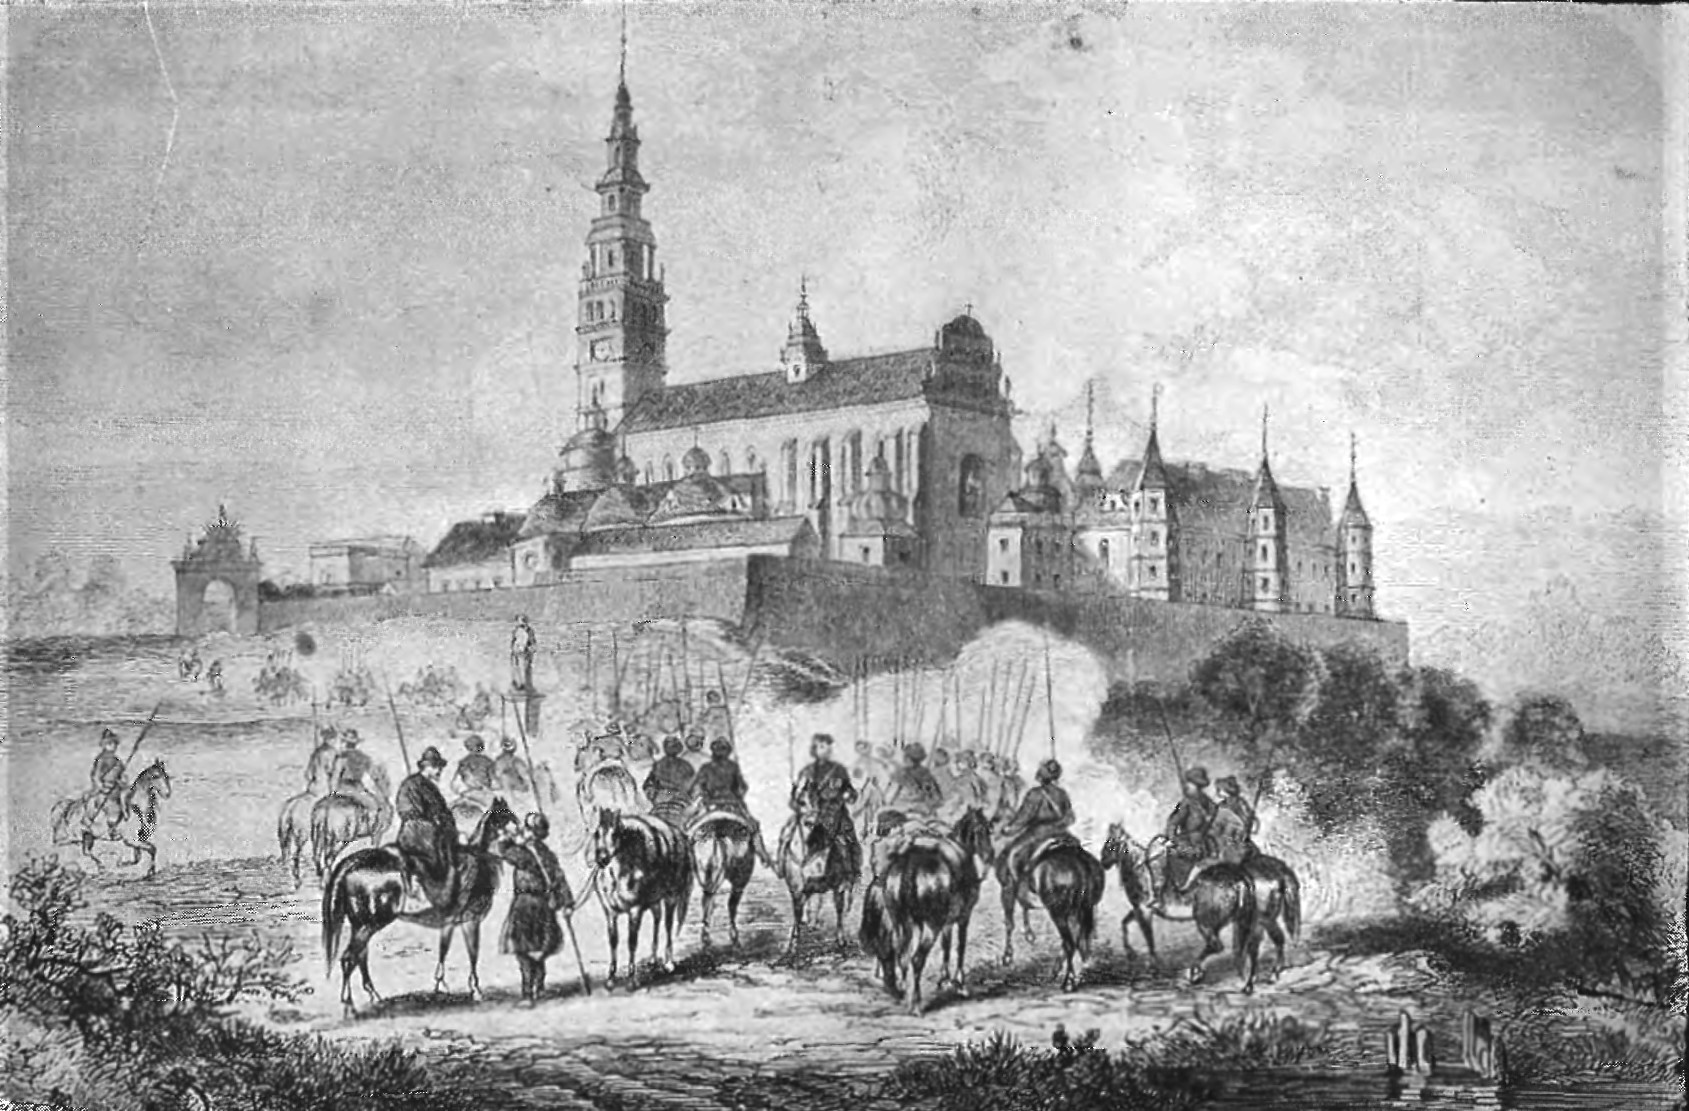
\includegraphics[width=\textwidth]{czestochowa.jpg}

\newpage

\setlength{\parskip}{1em}

\section{Appendix 1: The Pauline Collect Tone}

The Roman rite has two melodies for the Collect at Mass. A simple form and a Solemn form. Most Catholics would have heard the Solemn form and be familiar with it. The Pauline order has its own variation on the tone of the collect. This tone is  a part of the tradition and patrimony of the Order. It is quite beautiful and melodic. Below is the tone is its abstract form. 

\gregorioscore{../music/scheme}

For the benefit of a cantor or celebrant leading the Kneeling prayers, here are the 7 collects of the devotion written out fully in Gregorian notations with the Pauline collect tone applied. 

\gresetlastline{ragged}
\gresethyphen{auto}
\gresetinitiallines{0}
\gregorioscore{../music/orationes-i}
\medskip
\gresetinitiallines{1}
\gregorioscore{../music/orationes-ii}
\medskip
\gresetinitiallines{1}
\gregorioscore{../music/orationes-iii}
\medskip
\gresetinitiallines{1}
\gregorioscore{../music/orationes-iv}
\medskip
\gresetinitiallines{1}
\gregorioscore{../music/orationes-v-i}
\medskip
\gresetinitiallines{1}
\gregorioscore{../music/orationes-v-ii}
\medskip
\gresetinitiallines{1}
\gregorioscore{../music/orationes-vi}

\gregorioscore{../music/per-christum}

\newpage 

\noindent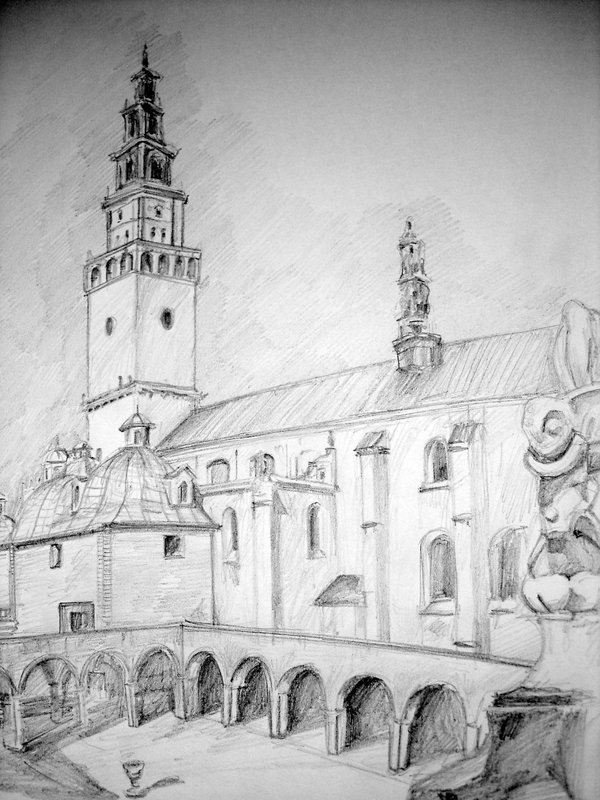
\includegraphics[width=\textwidth,height=\textheight]{jasna-gora}

\newpage 

\section{Appendix 2: Omni Die Dic Mariae}

\gresetlastline{justified}
\gresethyphen{force}
\gresetinitiallines{0}

\gregorioscore{../music/omni-die-dic-mariae-i}%
\begin{nstabbing}%
\>2. Con-tem-\>pla- re \>et \>mi- \hspace{1mm} ra- \hspace{1mm}re \>E- ius \>cel- \hspace{2mm} si-\>tu- di- nem, \\
\end{nstabbing}

\gregorioscore{../music/omni-die-dic-mariae-ii}%
\begin{nstabbing}%
\>Dic fe-\>li-cem \>Ge- ni-\>tri- \>cem, Dic \>be- \hspace{3mm} a- \>tam \>Vir- gi- nem. \\
\end{nstabbing}

\gregorioscore{../music/omni-die-dic-mariae-iii}%
\begin{nstabbing}%
\>4. Prop-ter \> Her-am \> ho-mo \hspace{2mm} sae- vam \>ac- \hspace{2mm} ce- \> pit \>sen- \>ten- ti- am; \\
\end{nstabbing}

\gregorioscore{../music/omni-die-dic-mariae-iv}%
\begin{nstabbing}%
\>Per \>Ma- ri- am \>ha- \hspace{1mm}bet \>vi- am, \>quae du- cit ad \>pa- tri- am. \\
\end{nstabbing}

\gregorioscore{../music/omni-die-dic-mariae-v}%
\begin{nstabbing}%
\>6. Vir- \hspace{1mm}ga \>Ies-se \>spes op- \>pres-sae \>men- tis \>et \>re-  \hspace{2mm} fu- \hspace{1mm} gi- um \\
\end{nstabbing}

\gregorioscore{../music/omni-die-dic-mariae-vi}%
\begin{nstabbing}%
\>De-cus \>mun-di \>lux pro-fun-di \>Do- mi- \>ni \>sa- cra- ri-um. \>A- men. \\
\end{nstabbing}

\newpage

\section*{Omni Die Dic Mariae}
\begin{multicols}{2}
\noindent Every day, my soul, \\
speak praises to Mary; \\
Her feasts and her feats \\
honour most devoutly. \par

\noindent Contemplate her and admire \\
her exaltation; \\
Say, “Happy Mother”; \\
say “Blessed Virgin.” \par

\noindent Honour her, \\
that she may free you \\
from your load of crimes; \\
Appeal to her, \\
lest a storm of vices \\
overcome you. \par

\noindent That I be chaste, modest, sweet, \\
mild, sober, Pious, righteous, \\
circumspect, ignorant of hostility, \par

\noindent Mercifully hear those whom you see \\
persisting in your praise; \\
Cleanse the guilty, and make them \\
worthy of heavenly gifts. \par

\noindent Holy Virgin, look at how many dangers we always meet, \\
so support us  \\
so that we are firm and vigorous. \par
\vspace*{2em}
\end{multicols}


\newpage

\section{Appendix 3: Maria Mater Gratiae}

\gresetlastline{justified}
\gresethyphen{force}
\gresetinitiallines{1}
\FDB{0}{\gregorioscore{../music/maria-mater-gratiae}}{
\section*{Maria Mater Gratiae}
\begin{center}
MARY, Mother of Grace,

Mother of mercy,

Shield me from the enemy

And receive me at the hour of my death.

\medskip

Glory to you, 

 Jesus, you who was born of the Virgin, 

With the Father and the Holy Spirit 

For every century. Amen.
\end{center}}

\newpage\null\newpage\null\thispagestyle{empty}\newpage


\end{document}
